\documentclass[12pt,a4paper]{article}
\usepackage[utf8]{inputenc}
\usepackage{graphicx}
\usepackage{tikz}
\usetikzlibrary{fit}
\usepackage{lmodern}
\usepackage{sectsty}
\usepackage{hyperref}


\sectionfont{\color{cyan}}

\begin{document}
   \begin{titlepage}
      {\fontfamily{lmss}\selectfont
      	\centering
      	
\includegraphics[width=0.30\textwidth]{logo.png}\par\vspace{1cm}
      	{\LARGE Compiax \par}
      	\vspace{0.25cm}
      	{\huge\bfseries \color{cyan}SplitBill\par}
      	\vspace{1cm}
      	{\Large\textit{by} Brute Force\par}
         \vspace{0.25cm}
         \begin{tikzpicture}
            \node [inner sep=0pt,,outer sep=0pt,clip,rounded corners=0.5cm] (pict) at (0,0) {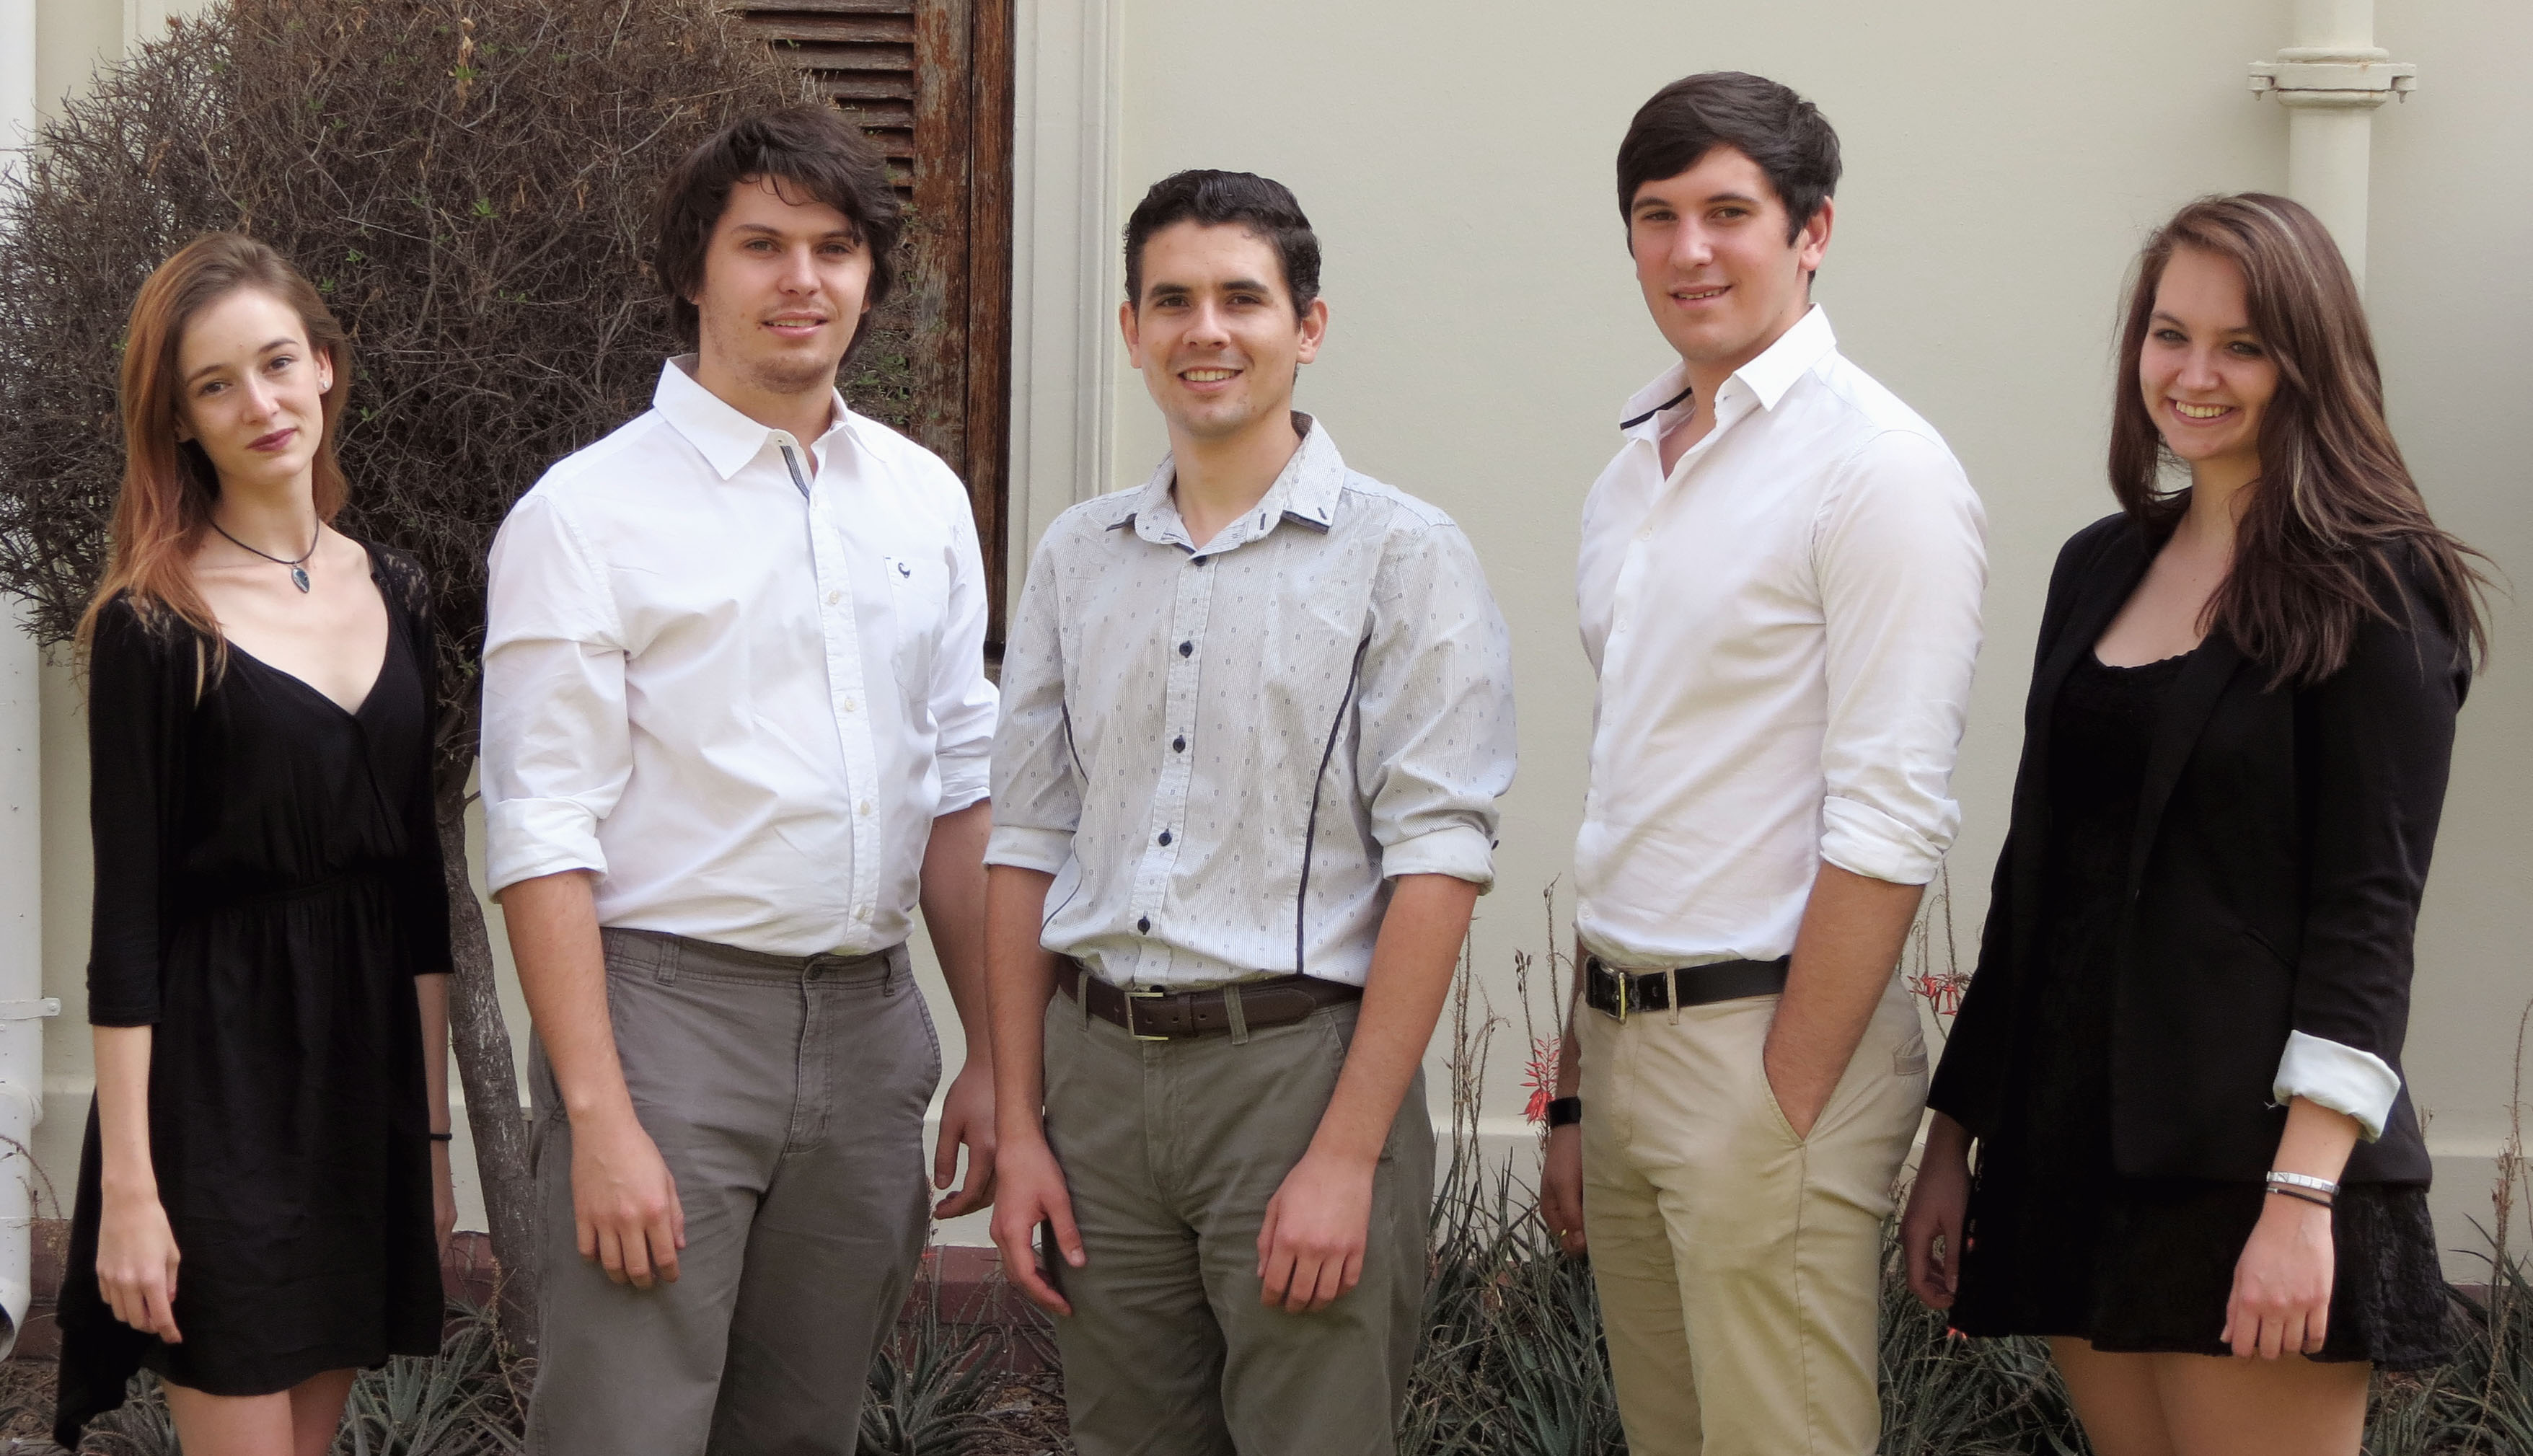
\includegraphics[width=0.9\textwidth]{team.jpg}};
            \node[fit=(pict),rounded corners=.55cm,inner sep=2pt]{};
         \end{tikzpicture}

         \par\vspace{1cm}
         \date{}
         \author{}
         \title{}
         \centering
         \textbf{Authors:}\\
         Mia Gerber\\
         Matthew Perry\\
         Wanrick Willemse\\
         Duart Breedt\\
         Linda Potgieter\\
      }
   \end{titlepage}
   \maketitle
   \tableofcontents
   \newpage

   \section{Introduction}
   The project presented is the development of a mobile application that will manage the division of items on a restaurant receipt among the patrons around the table. We believe this product can be extended to manage
   collective shopping receipts and essentially any receipt that contains items that needs to be split among users. This document serves as our proposal of how to address this issue.

   \section{Project description}
   At the highest level our objective is to create a user friendly app, that is visually appealing and enjoyable to use. The following high level requirements are to be met:
   \begin{itemize}
      \item \textbf{Capture and interpret the receipt}\\
         For this we are considering Tesseract-OCR.\@ Tesseract is an open-source OCR library, sponsored by Google. Mobile libraries exist for both Andriod and iOS.\@ This can be used with no charge.\\
         An alternative would be Google's Mobile Vision API.\@ This however comes with some limitations with regards to daily usage and fees may be incurred with a large user base. For development and testing purposes, this
         should not be a problem.
      \item \textbf{Add users}\\
         One user will be required to take a photo of the receipt. This user will act as the host of the session. By using NFC or QR scan other users will be added to the bill. If a user does not have the app installed, any
         other user will be allowed to add a `guest' whose bill can then be calculated.
      \item \textbf{Provide an interface}\\
         The app interface will be built using AngularJS and Ionic. This will ensure a cross-platform application.
      \item \textbf{Live sync}\\
         For offline sync we are looking into Couchbase lite to handle peer to peer replication. Couchbase is fully integratable into the MEAN stack essentially replacing MongoDB.\@ Authentication and connection information can
         then be tranferred using NFC or a QR barcode.\\
         Using MongoDB may require internet access when syncing in real time.\\
         Bluetooth is also very limited in the amount of devices it allows and currently compatibility between Android and iOS bluetooth devices is questionable at best.
      \item \textbf{Learn}\\
         Adding functionality for learning new receipt formats will be done by extending the user interface and further utilizing the OCR component. Input from the user will divide the image into the appropriate fields and the
         format can be stored in JSON format.
      \item \textbf{App and server}\\
         Server functionality will be useful for centralizing the formats of receipts, and result in a smaller app size if the format of a receipt is fetched from an online database. As a team we agree that the pros and cons of
         using a server must be carefully considered. We intend to make the application as cost-effective as possible.
   \end{itemize}
   Basic planned functionality is as follows. A user takes a picture of the receipt and this is processed and represented on the user interface. The user is then given the option to invite other to join this receipt. Checkboxes
   next to items allow users to claim items and a subtotal is generated for each user. Each user is then given the opportunity to add a tip. On each device the total for the receipt is displayed, as well as the subtotal for the
   specific user and the total that the group's contributions amount to.

   \clearpage
   \subsection{Deployment Diagram}
   \begin{figure}[h]
   \center
   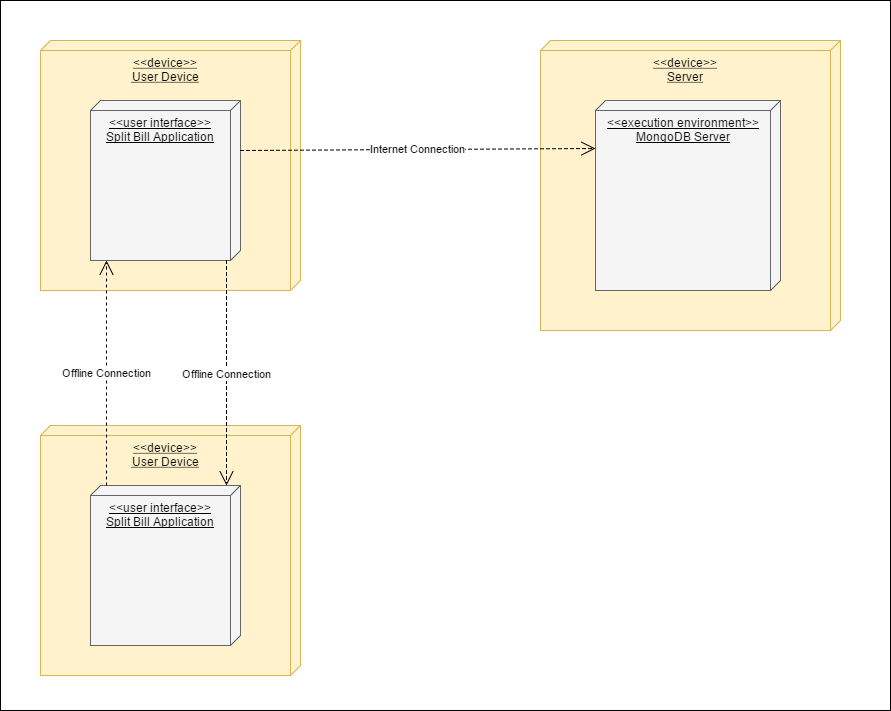
\includegraphics[width=0.98\textwidth]{SplitBill_deployment.png}
   \caption{Deployment Diagram}
   \end{figure}
   \newpage
   \section{Development Methodologies}
   \subsection{Interaction between development team and client}
   Primarily we believe our client to be the expert and we aim to meet the needs stipulated to us, in an accurate and timely manner. Not only to build a good quality product, but a useful one. With SplitBill we will rely on our
   collective knowledge and experience, the client's and our team's, to create a useful receipt sharing solution. A detailed expectation breakdown will be discussed if we are given this opportunity.

   Our team will strictly adhere to Agile Development Principles. The client will primarily be involved in testing and the feedback will serve as reference for future releases. It is important to us that the scope of the product
   is discussed and agreed upon by both the client, and our team. We are aware that requirements may change, but to ensure that a quality, useful product results from the available time-frame, we prefer to have an agreed upon
   feature list to direct our course.

   \subsection{Interaction between members of development team}
   Our team will apply SCRUM methodologies in order to structure how teamwork will occur for this project, this is a faster, more intensely iterative approach to controlling workflow.

   We are using Slack and ZenHub (in conjunction with GitHub) to ensure that team members are aware of each other even when we are not physically together and are alerted when work is either available or completed.
	Meetings will be held once a week regardless of the state of the project. Each meeting will require that each team member give a small summary of work done that week, enforcing accountability.
   Working in weekly `sprints' also optimizes predictability and minimizes risk (if something does go wrong it is only a week's worth of work lost, not a whole month.)

   As a team we are going to be adhering to a practice called `pair-programming' which is essentially two or more people working on the same piece of code or feature in order to maximize the chances of bugs
   being discovered and minimize the time required to get a feature ready for production.

   \newpage
   \section{Our Team}
		\parbox[c][4cm]{4cm}{\tikz\node[circle,draw,minimum size=3.5cm, 
			path picture={
               \node at (path picture bounding box.center){
                   
\includegraphics[width=3.5cm]{mia.jpg}
               };
           }]{};
		}
		\parbox[c][4cm]{10cm}{\subsection*{Mia Gerber}B.IS Multimedia}\\\\
Logical thinking and reasoning has always come naturally to me, I enjoy being posed a question or problem and then left to use the tools at my disposal to answer and/or solve it.\\\\
I am stubborn in the pursuit of success, which leads to many hours being sunk into troubleshooting if a product or deliverable does not meet all the requirements.\\\\
I am skilled in both the technical and creative side of development, in other words, formulating somewhat unconventional solutions and then executing them in a professional manner.\\\\
I believe that my team members and I are capable of making this project a success through our already existing abilities as well as sheer tenacity.\\\\
		\textbf{\small Experience and Project:}\\
		University of Pretoria’s EBIT Week IT team\\
		eCommerce website (both front and backend development) as undergraduate project\\
		Teaching Assistant for the Computer Science department\\\\
		\parbox{\textwidth}{
			\textbf{\small Relevant skills:}
			\begin{itemize}\itemsep0em
				\item Programming Languages:
				\begin {itemize}\itemsep0em
					\item C++
					\item C
					\item C\#
					\item Java
					\item x86 Assembly Language
					\item Javascript
					\item JQuery
					\item Actionscript 3.0
				\end {itemize}
				\item Markup Languages:
				\begin {itemize}\itemsep0em
					\item XML
					\item HTML
					\item JSON
					\item CSS
					\item Bootstrap
				\end {itemize}
				\item Frameworks:
				\begin {itemize}\itemsep0em
					\item MEAN stack development
					\begin {itemize}\itemsep0em
						\item Node.js
						\item Angular.js
						\item Express.js
						\item MongoDB
					\end {itemize}
					\item LAMP stack development
					\begin {itemize}\itemsep0em
						\item MySQL
						\item PostgreSQL
						\item PHP
					\end {itemize}
				\end {itemize}
				\item Software:
				\begin {itemize}\itemsep0em
					\item Adobe Creative Suite
					\item Modelio
				\end {itemize}
			\end{itemize}
		}
		\newpage
		\parbox[c][4cm]{4cm}{\tikz\node[circle,draw,minimum size=3.5cm, 
			path picture={
               \node at (path picture bounding box.center){
                   
\includegraphics[width=3.5cm]{matthew.jpg}
               };
           }]{};
		}
		\parbox[c][4cm]{10cm}{\subsection*{Matthew Perry}B.Sc IT GIS}\\\\
		I am passionate about software development. Being able to write code to solve a problem excites me. I am driven to be able to learn new technologies and be able to use them to create software and solve problems. I am a critical thinker that thrives when given something complex to assess and work on.
I am able to work well under pressure and ensure that the final result exceeds expectations. I can adapt to the situation so that I can perform at my peak. Learning and gathering experience are very important aspects in my life.\\\\
		\textbf{\small Experience and Project:}\\
		HCI task to redesign an app to improve user experience.\\
		Programmed an FPGA board using VHDL.\\\\
		\parbox{\textwidth}{
			\textbf{\small Relevant skills:}\\
			\parbox{5cm}{
				\begin{itemize}\itemsep0em
					\item OOP
					\begin {itemize}\itemsep0em
						\item C++
						\item Java
						\item Python
						\item Javascript
					\end {itemize}
				\end {itemize}
			} 
			\parbox{5cm}{
				\begin{itemize}\itemsep0em	
					\item Web Development
					\begin {itemize}\itemsep0em
						\item HTML
						\item PHP
						\item NodeJS
						\item SQL
						\item MongoDB
					\end {itemize}
				\end {itemize}
			}
			\begin{itemize}\itemsep0em	
				\item C
				\item Android Studio
				\item Hardware Descriptive Language: VHDL
				\item Cisco CCNA 6.0 and CCNP Route qualifications
				\item GIS (ArcGIS, QGIS)
			\end{itemize}
		}
		\newpage
		\parbox[c][4cm]{4cm}{\tikz\node[circle,draw,minimum size=3.5cm, 
			path picture={
               \node at (path picture bounding box.center){
                   
\includegraphics[width=3.5cm]{wanrick.jpg}
               };
           }]{};
		}
		\parbox[c][4cm]{10cm}{\subsection*{Wanrick Willemse}B.IS Multimedia}\\\\
		I’ve always enjoyed finding a solution to a challenge. I believe that anything can be overcome if it is approached systematically and with determination.\\\\
Meticulous design and thorough planning should be at the forefront of tackling a problem. I try to establish a vision and use it as a roadmap when creating something. I consider a product successful when I can see it is of a high standard.\\\\
I am adaptable and can function well under pressure. When it comes to my work, there is no settling for second best.\\\\
Developing high-quality software expects no less.\\\\
		\textbf{\small Experience and Project:}\\
		7 years work experience at a pathology company\\
		eCommerce website as undergraduate project\\
		Tutor for first year webdesign and second year Visual Design\\\\
		\parbox{\textwidth}{
			\textbf{\small Relevant skills:}
			\begin{itemize}\itemsep0em
				\item OOP and Procedural programming in: C++, C, Java, PHP, Python and JavaScript
				\item Web Development: HTML, CSS, Bootstrap, MEAN and LAMP stack
				\item XML, JSON and WebGL
				\item Adobe Suite, HCI, UX and UI design
			\end{itemize}
		}
		\newpage
		\parbox[c][4cm]{4cm}{\tikz\node[circle,draw,minimum size=3.5cm, 
			path picture={
               \node at (path picture bounding box.center){
                   
\includegraphics[width=3.5cm]{duart.jpg}
               };
           }]{};
		}
		\parbox[c][4cm]{10cm}{\subsection*{Duart Breedt}B.IS Multimedia}\\\\
		I take pride in making all my work aesthetically pleasing and believe it is of the utmost importance that all user-centered products should have great UI and UX design.\\\\
I think of myself as a perfectionistic completionist. Characteristically, I work persistently on any endeavour I undertake until I have produced a quality product I am proud of.\\\\
\parbox{\textwidth}{I find that if I am not learning, I am bored. Therefore, I strive to seek out challenges which push my limits and force me to contend with steep learning curves.\\}
I strongly believe that if you ever wish to be great at what you do you should ensure you are never the smartest person in the room. People are vessels of knowledge and will teach you more than you would like to know if you let them.\\\\
		\textbf{\small Experience and Projects (Please see my LinkedIn and GitHub for more detail):}\\
		Developed a website for Caelum Technologies\\
		Developing a website for the National Field Trial Association\\
		Developing a website for TallTrees Learning Community\\
		\href{http://77-breedt.000webhostapp.com}{Developed an ecommerce website as an undergraduate based project}\\\\
		\parbox{\textwidth}{		
			\textbf{\small Relevant skills:}
			\begin{itemize}\itemsep0em
				\item Object-Oriented Programming
				\item Java
				\item C++
				\item XML
				\item JSON
				\item Web Development:
				\begin {itemize}\itemsep0em
					\item HTML
					\item CSS
					\item Bootstrap
					\item Javascript
					\item JQuery
					\item MEAN stack (NodeJS, MongoDB, AngularJS)
					\item LAMP stack (PHP, SQL)
				\end {itemize}
				\item Design principles (UI, UX, HCI)
				\item Visual Design
				\item Adobe Creative Suite

			\end{itemize}
		}
		\newpage
		\parbox[c][4cm]{4cm}{\tikz\node[circle,draw,minimum size=3.5cm, 
			path picture={
               \node at (path picture bounding box.center){
                   
\includegraphics[width=3.5cm]{linda.jpg}
               };
           }]{};
		}
		\parbox[c][4cm]{10cm}{\subsection*{Linda Potgieter}B.Sc IT Genetics}\\\\
		I am always up for a challenge. Nothing great is worth achieving by taking the easy way out.. I am always analyzing the problem to ensure I find the most effective but easiest to understand solution.\\\\
I am always willing to find a solution to a problem on my own, but I know when I need to ask for assistance. Struggling alone is not an option when project quality is at stake. Strong believer in the use and creation of complete and concise documentation for any project. \\\\
I perform well under pressure, but ensure the pressure placed on myself with regards to my studies is at minimum by setting milestones and achieving them within a set timeframe. No one likes sloppy last minute work, and clients deserve more than that, even if it is only a teaching assistant assessing the work.\\\\
		\textbf{\small Experience and Project:}\\
		Redesign of mobile application to comply with HCI standards as undergraduate project.\\\\
		\parbox{\textwidth}{
			\textbf{\small Relevant skills:}
			\begin{itemize}\itemsep0em
				\item Java
				\item Python
				\item C++
				\item x86 Assembly Language 
				\item JSON
				\item Web development
				\begin {itemize}\itemsep0em
					\item HTML
					\item CSS
					\item Bootstrap
					\item XML
					\item JavaScript
					\item JQuery
					\item MEAN Stack
					\begin {itemize}\itemsep0em
						\item AngularJS
						\item NodeJS
						\item MongoDB
						\item ExpressJS
					\end {itemize}
					\item LAMP stack
					\begin {itemize}\itemsep0em
						\item PHP
						\item SQL (MySQL and MSQL)
					\end {itemize}
				\end {itemize}
				\item Design principles
				\item Human Computer Interaction design
				\item User interface design
				\item User experience design
				\item Other 
				\begin {itemize}\itemsep0em
					\item Genome analysis programs 
					\begin {itemize}\itemsep0em
						\item MEGA 6.06
						\item Mothur
						\item MCRobot
					\end {itemize}
				\end {itemize}
			\end{itemize}
		}
\end{document}
